\documentclass[aspectratio=169]{beamer}

\mode<presentation>
{
  \usetheme{default}
  \usecolortheme{default}
  \usefonttheme{default}
  \setbeamertemplate{navigation symbols}{}
  \setbeamertemplate{caption}[numbered]
  \setbeamertemplate{footline}[frame number]  % or "page number"
  \setbeamercolor{frametitle}{fg=white}
  \setbeamercolor{footline}{fg=black}
} 

\usepackage[english]{babel}
\usepackage[utf8x]{inputenc}
\usepackage{tikz}
\usepackage{courier}
\usepackage{array}
\usepackage{bold-extra}
\usepackage{minted}
\usepackage[thicklines]{cancel}

\xdefinecolor{dianablue}{rgb}{0.18,0.24,0.31}
\xdefinecolor{darkblue}{rgb}{0.1,0.1,0.7}
\xdefinecolor{darkgreen}{rgb}{0,0.5,0}
\xdefinecolor{darkgrey}{rgb}{0.35,0.35,0.35}
\xdefinecolor{darkorange}{rgb}{0.8,0.5,0}
\xdefinecolor{darkred}{rgb}{0.7,0,0}
\definecolor{darkgreen}{rgb}{0,0.6,0}
\definecolor{mauve}{rgb}{0.58,0,0.82}

\title[2017-11-16-dataorg-columnar]{Managing data with columnar granularity}
\author{Jim Pivarski}
\institute{Princeton University -- DIANA-HEP}
\date{November 16, 2017}

\begin{document}

\logo{\pgfputat{\pgfxy(0.11, 7.4)}{\pgfbox[right,base]{\tikz{\filldraw[fill=dianablue, draw=none] (0 cm, 0 cm) rectangle (50 cm, 1 cm);}\mbox{\hspace{-8 cm}
\includegraphics[height=1 cm]{princeton-logo-long.png}
\includegraphics[height=1 cm]{diana-hep-logo-long.png}}}}}

\begin{frame}
  \titlepage
\end{frame}

\logo{\pgfputat{\pgfxy(0.11, 7.4)}{\pgfbox[right,base]{\tikz{\filldraw[fill=dianablue, draw=none] (0 cm, 0 cm) rectangle (50 cm, 1 cm);}\mbox{\hspace{-8 cm}
\includegraphics[height=1 cm]{princeton-logo.png}
\includegraphics[height=1 cm]{diana-hep-logo.png}}}}}

% Uncomment these lines for an automatically generated outline.
%\begin{frame}{Outline}
%  \tableofcontents
%\end{frame}

% START START START START START START START START START START START START START

\begin{frame}{Nature of this talk}
\vspace{0.5 cm}
\begin{columns}
\column{1.05\linewidth}
\Large This talk isn't about how we manage data in HEP, but how we {\it might.}
\end{columns}

\vspace{0.5 cm}
\begin{itemize}\setlength{\itemsep}{0.25 cm}
\item \Large Therefore, it isn't a ``how-to'' talk but a ``what-if'' talk.
\item \Large If you have experience in this, we want to hear from you!
\end{itemize}
\end{frame}

\begin{frame}{Columnar data}
\vspace{0.35 cm}
\begin{columns}
\column{0.45\linewidth}
Serializing data in columns is an old idea in HEP:

\vspace{0.25 cm}
\begin{itemize}
\item \textcolor{darkblue}{1989:} Column-Wise-N-tuples (CWN) in PAW
\item \textcolor{darkblue}{1996:} ``split'' (columnar) C++ objects in ROOT

\vspace{0.25 cm}
\ldots

\vspace{0.25 cm}
\item \textcolor{darkblue}{2002:} MonetDB
\item \textcolor{darkblue}{2005:} C-Store (Vertica)
\item \textcolor{darkblue}{2010:} Google Dremel paper
\item \textcolor{darkblue}{2013:} Apache Parquet
\item \textcolor{darkblue}{2016:} Apache Arrow
\end{itemize}

\column{0.55\linewidth}
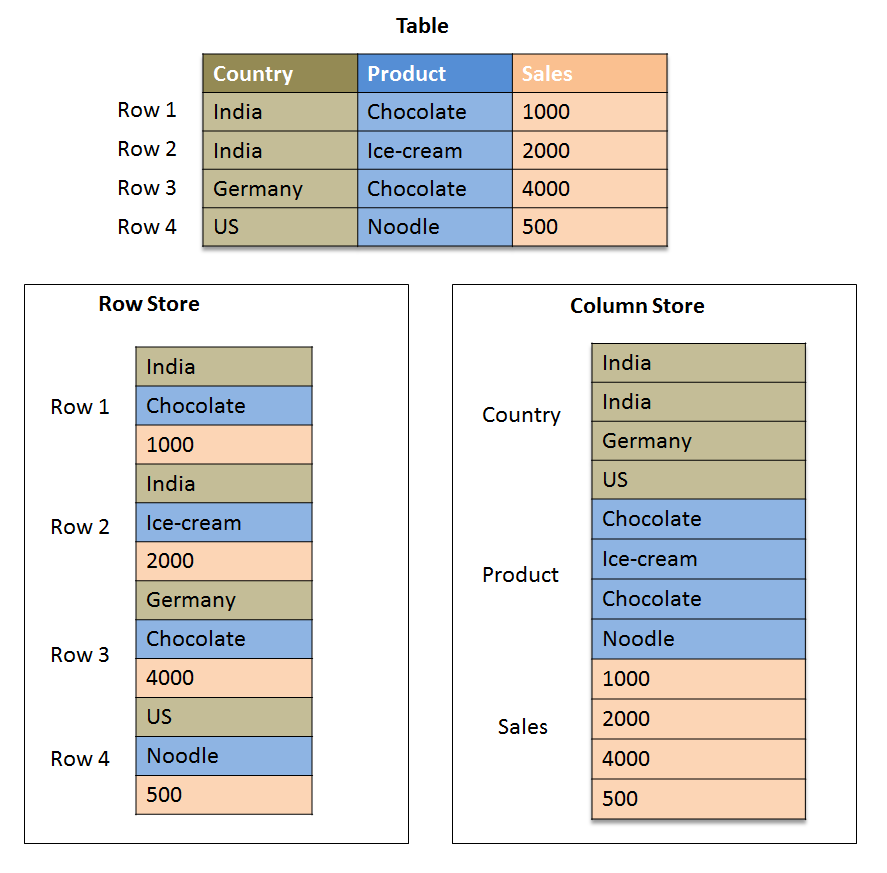
\includegraphics[width=\linewidth]{columnar-vs-rowwise-sap.png}
\end{columns}
\end{frame}

\begin{frame}{Hierarchically nested columnar data}
\vspace{0.25 cm}
Rowwise $\to$ columnar is a transposition for tabular data; nested data is more complex.

\begin{uncoverenv}<2->
\vspace{0.25 cm}
\textcolor{darkblue}{Example:} {\tt\small vector<vector<pair<char, int>>>}

\vspace{0.25 cm}
\begin{tabular}{r l}
\small logical data & {\tt\scriptsize \textcolor{blue}{[}\textcolor{violet}{[}(\textcolor{darkorange}{a},\textcolor{darkgreen}{1}), (\textcolor{darkorange}{b},\textcolor{darkgreen}{2}), (\textcolor{darkorange}{c},\textcolor{darkgreen}{3}), (\textcolor{darkorange}{d},\textcolor{darkgreen}{4})\textcolor{violet}{]}, \textcolor{violet}{[]}, \textcolor{violet}{[}(\textcolor{darkorange}{e},\textcolor{darkgreen}{5}), (\textcolor{darkorange}{f},\textcolor{darkgreen}{6})\textcolor{violet}{]}\textcolor{blue}{]}, \textcolor{blue}{[]}, \textcolor{blue}{[}\textcolor{violet}{[}(\textcolor{darkorange}{g},\textcolor{darkgreen}{7})\textcolor{violet}{]}\textcolor{blue}{]}\ \textcolor{white}{]}} \\\hline
\small outer stops & {\tt\scriptsize \textcolor{blue}{[\ \ \ \ \ \ \ \ \ \ \ \ \ \ \ \ \ \ \ \ \ \ \ \ \ \ \ \ \ \ \ \ \ \ \ \ \ \ \ \ \ \ \ \ \ \ \ \ 3,\ \ 3,\ \ \ \ \ \ \ \ \ 4]}} \\
\small inner stops & {\tt\scriptsize \textcolor{violet}{[\ \ \ \ \ \ \ \ \ \ \ \ \ \ \ \ \ \ \ \ \ \ \ \ \ \ \ 4,\ \ 4,\ \ \ \ \ \ \ \ \ \ \ \ \ \ 6,\ \ \ \ \ \ \ \ \ \ \ \ \ 7\ ]}} \\
\small 1$^{\mbox{\scriptsize st}}$ attribute & {\tt\scriptsize \textcolor{darkorange}{[\ \ a,\ \ \ \ \ b,\ \ \ \ \ c,\ \ \ \ \ d,\ \ \ \ \ \ \ \ \ \ \ e,\ \ \ \ \ f,\ \ \ \ \ \ \ \ \ \ \ \ \ g\ \ \ \ \ ]}} \\
\small 2$^{\mbox{\scriptsize nd}}$ attribute & {\tt\scriptsize \textcolor{darkgreen}{[\ \ \ \ 1,\ \ \ \ \ 2,\ \ \ \ \ 3,\ \ \ \ \ 4,\ \ \ \ \ \ \ \ \ \ \ 5,\ \ \ \ \ 6,\ \ \ \ \ \ \ \ \ \ \ \ \ 7\ \ \ ]}}
\end{tabular}
%% \begin{tabular}{r l}
%% \small logical data & {\tt\scriptsize \textcolor{white}{[}\textcolor{blue}{[}\textcolor{violet}{[}(\textcolor{darkorange}{a},\textcolor{darkgreen}{1}), (\textcolor{darkorange}{b},\textcolor{darkgreen}{2}), (\textcolor{darkorange}{c},\textcolor{darkgreen}{3}), (\textcolor{darkorange}{d},\textcolor{darkgreen}{4})\textcolor{violet}{]}, \textcolor{violet}{[]}, \textcolor{violet}{[}(\textcolor{darkorange}{e},\textcolor{darkgreen}{5}), (\textcolor{darkorange}{f},\textcolor{darkgreen}{6})\textcolor{violet}{]}\textcolor{blue}{]}, \textcolor{blue}{[]}, \textcolor{blue}{[}\textcolor{violet}{[}(\textcolor{darkorange}{g},\textcolor{darkgreen}{7})\textcolor{violet}{]}\textcolor{blue}{]}\ \textcolor{white}{]}} \\\hline
%% \small outer offsets & {\tt\scriptsize \textcolor{blue}{[0,\ \ \ \ \ \ \ \ \ \ \ \ \ \ \ \ \ \ \ \ \ \ \ \ \ \ \ \ \ \ \ \ \ \ \ \ \ \ \ \ \ \ \ \ \ \ \ \ \ \ 3,\ \ 3,\ \ \ \ \ \ \ 4]}} \\
%% \small inner offsets & {\tt\scriptsize \textcolor{violet}{[\ 0,\ \ \ \ \ \ \ \ \ \ \ \ \ \ \ \ \ \ \ \ \ \ \ \ \ \ \ \ 4,\ \ 4,\ \ \ \ \ \ \ \ \ \ \ \ \ \ \ \ \ \ \ \ 6,\ \ \ \ \ \ 7]}} \\
%% \small 1$^{\mbox{\scriptsize st}}$ attribute & {\tt\scriptsize \textcolor{darkorange}{[\ \ \ a,\ \ \ \ \ b,\ \ \ \ \ c,\ \ \ \ \ d,\ \ \ \ \ \ \ \ \ \ \ e,\ \ \ \ \ f,\ \ \ \ \ \ \ \ \ \ \ \ \ g\ \ \ \ \ \ ]}} \\
%% \small 2$^{\mbox{\scriptsize nd}}$ attribute & {\tt\scriptsize \textcolor{darkgreen}{[\ \ \ \ \ 1,\ \ \ \ \ 2,\ \ \ \ \ 3,\ \ \ \ \ 4,\ \ \ \ \ \ \ \ \ \ \ 5,\ \ \ \ \ 6,\ \ \ \ \ \ \ \ \ \ \ \ \ 7\ \ \ \ ]}}
%% \end{tabular}
\end{uncoverenv}

\begin{itemize}
\item<3-> Each primitive attribute is in an array by itself, with no list boundaries.
\item<4-> Stops array: cumulative number of items for some level at each {\it closing} bracket.
\item<5-> \textcolor{darkblue}{Alternative representations:}
\begin{itemize}
\item<5-> Offsets (Arrow): include {\it starting} index; can represent interval slices without copying.
\item<6-> Starts and stops: {\tt\scriptsize starts, stops = offsets[:-1], offsets[1:]}; can represent union of interval slices without copying, even save out of order for indexed lookups.
\item<7-> Sizes: {\tt\scriptsize sizes = stops - starts}; compressible, fill in parallel, but no $\mathcal{O}(1)$ lookup.
\item<8-> Dremel/Parquet: ``repetition level''; packed small integers, but no $\mathcal{O}(1)$ lookup.
\end{itemize}
%% \item<4-> Offset array: starting index of nested data at each open bracket; total size at end.
%% \item<5-> Alternate representations:
%% \begin{itemize}
%% \item<5-> stops: {\tt\scriptsize stops = offsets[1:]} (one value per item; can't drop prefix without a copy)
%% \item<6-> starts and stops: {\tt\scriptsize starts = offsets[:-1]; stops = offsets[1:]} (full slicing, including arbitrary skips, without a copy; even save out of order for indexed lookups)
%% \item<7-> sizes: {\tt\scriptsize sizes = stops - starts} (compressible; create in parallel; can't $\mathcal{O}(1)$ lookup)
%% \item<8-> Dremel/Parquet: ``repetition level'' (packed small integers; can't $\mathcal{O}(1)$ lookup)
%% \end{itemize}
\end{itemize}
\end{frame}

\begin{frame}{}
\begin{center}
\begin{minipage}{0.8\linewidth}
\begin{center}
\Large Although we know how to save and retrieve data in columnar form, we still manage data {\it as files.}
\end{center}
\end{minipage}
\end{center}

\vspace{0.5 cm}
Whether it's ROOT or Parquet, a file structure glues a set of columns together to be downloaded, replicated, versioned, or migrated to colder storage {\it as a unit.}
\end{frame}

\begin{frame}{Why is this a problem?}
\vspace{0.5 cm}
\textcolor{darkblue}{The reason columnar data is so useful is because each end-user analysis requires a minority of the data columns.}

\vspace{0.25 cm}
\begin{uncoverenv}<2->
\begin{center}
\begin{minipage}{0.9\linewidth}
\begin{itemize}
\item ``Monojet analysis'' \textcolor{gray}{only needs jet objects, but it needs jets constructed many different ways to study systematics.}
\item ``Boosted top search'' \textcolor{gray}{needs jets with substructure variables.}
\item ``Heavy flavor study'' \textcolor{gray}{needs jets, electrons, and muons with isolation and B-tagging variables.}
\item ``Diphoton Higgs mass'' \textcolor{gray}{needs photons, electrons for a veto, and converted pair electrons.}
\item \ldots
\end{itemize}
\end{minipage}
\end{center}
\end{uncoverenv}

\vspace{0.25 cm}
\uncover<3->{Within each particle object, the kinematic variables ($p_T$, $\eta$, $\phi$, $m$) are needed the most, with ``isolation/tagging/matching/\ldots'' needed by different analyses \mbox{to varying degrees.\hspace{-1 cm}}}

\begin{uncoverenv}<4->
\vspace{-5 cm}
\begin{center}
\fcolorbox{black}{white}{\begin{minipage}{0.9\linewidth}
\vspace{0.5 cm}
\begin{center}
\begin{minipage}{0.95\linewidth}
Columnar data lets us read relevant attributes from disk (or with XRootD, over the network) one at a time, but our data management systems are unaware of how to open up a ROOT file and operate on individual columns.
\end{minipage}
\end{center}
\vspace{0.2 cm}
\end{minipage}}
\end{center}
\vspace{5 cm}
\end{uncoverenv}
\end{frame}

\begin{frame}{What could we do if data management were column-aware?}
\vspace{0.15 cm}
\mbox{\hspace{-0.5 cm}\begin{columns}
\column{1.1\linewidth}
\begin{description}\setlength{\itemsep}{0.2 cm}
\item[Case 1:]<1-> \textcolor{darkblue}{serve most desirable attributes from RAM or SSD and less desirable attributes of the same dataset from disk or tape.}

\vspace{0.2 cm}
Currently, we make 2 or 3 levels of ``slimmed'' copies (AOD/MiniAOD/NanoAOD) to serve with different latencies. Three sizes does not fit all, so individual analyses make their own subsets (and have to find storage on their own).

\item[Case 2:]<2-> \textcolor{darkblue}{define datasets with overlapping sets of physical columns.}

\vspace{0.2 cm}
For instance, version~1 has incorrect jet energy corrections; version~2 is just like it but with different jet energies. Versions~1 and 2 should point to the same data and share storage for all other columns. (Currently, users distribute recipes!)

\item[Case 3:]<3-> \textcolor{darkblue}{provide zero-copy views of selected particles or events through stencils/bitmaps.}

\vspace{0.2 cm}
Currently, users make ``skimmed'' copies, which use more space and can't benefit from version updates such as the jet energy correction example above.

\item[Case 4:]<4-> \textcolor{darkblue}{accelerate selections with database-style indexing.}
\end{description}
\end{columns}}
\end{frame}

\begin{frame}{Case 1: lower latency for popular columns}
\vspace{0.5 cm}

\begin{tabular}{r l}
\small logical data & {\tt\scriptsize \textcolor{blue}{[}\textcolor{violet}{[}(\textcolor{darkorange}{a},\textcolor{darkgreen}{1}), (\textcolor{darkorange}{b},\textcolor{darkgreen}{2}), (\textcolor{darkorange}{c},\textcolor{darkgreen}{3}), (\textcolor{darkorange}{d},\textcolor{darkgreen}{4})\textcolor{violet}{]}, \textcolor{violet}{[]}, \textcolor{violet}{[}(\textcolor{darkorange}{e},\textcolor{darkgreen}{5}), (\textcolor{darkorange}{f},\textcolor{darkgreen}{6})\textcolor{violet}{]}\textcolor{blue}{]}, \textcolor{blue}{[]}, \textcolor{blue}{[}\textcolor{violet}{[}(\textcolor{darkorange}{g},\textcolor{darkgreen}{7})\textcolor{violet}{]}\textcolor{blue}{]}\ \textcolor{white}{]}} \\\hline
\small outer stops & {\tt\scriptsize \textcolor{blue}{[\ \ \ \ \ \ \ \ \ \ \ \ \ \ \ \ \ \ \ \ \ \ \ \ \ \ \ \ \ \ \ \ \ \ \ \ \ \ \ \ \ \ \ \ \ \ \ \ 3,\ \ 3,\ \ \ \ \ \ \ \ \ 4]}} \\
\small inner stops & {\tt\scriptsize \textcolor{violet}{[\ \ \ \ \ \ \ \ \ \ \ \ \ \ \ \ \ \ \ \ \ \ \ \ \ \ \ 4,\ \ 4,\ \ \ \ \ \ \ \ \ \ \ \ \ \ 6,\ \ \ \ \ \ \ \ \ \ \ \ \ 7\ ]}} \\
\small 1$^{\mbox{\scriptsize st}}$ attribute & {\tt\scriptsize \textcolor{darkorange}{[\ \ a,\ \ \ \ \ b,\ \ \ \ \ c,\ \ \ \ \ d,\ \ \ \ \ \ \ \ \ \ \ e,\ \ \ \ \ f,\ \ \ \ \ \ \ \ \ \ \ \ \ g\ \ \ \ \ ]}} \\
\small 2$^{\mbox{\scriptsize nd}}$ attribute & {\tt\scriptsize \textcolor{darkgreen}{[\ \ \ \ 1,\ \ \ \ \ 2,\ \ \ \ \ 3,\ \ \ \ \ 4,\ \ \ \ \ \ \ \ \ \ \ 5,\ \ \ \ \ 6,\ \ \ \ \ \ \ \ \ \ \ \ \ 7\ \ \ ]}}
\end{tabular}

\vspace{0.5 cm}
If the numbers are more popular than the letters, raise the 2$^{\mbox{\scriptsize nd}}$ attribute into warmer cache (on the server) independently of the letters.

\vspace{0.5 cm}
To the degree that analysts' interests overlap (e.g.\ the all-popular kinematic variables), a copy in hot cache may be shared by all. This is impossible for private skims.
\end{frame}

\begin{frame}[fragile]{Case 2: overlapping dataset definitions}
\vspace{1 cm}

\begin{columns}
\column{1.05\linewidth}
\begin{tabular}{r l}
\small logical data & {\tt\scriptsize \textcolor{blue}{[}\textcolor{violet}{[}(\textcolor{darkorange}{a},\textcolor{darkgreen}{1}), (\textcolor{darkorange}{b},\textcolor{darkgreen}{2}), (\textcolor{darkorange}{c},\textcolor{darkgreen}{3}), (\textcolor{darkorange}{d},\textcolor{darkgreen}{4})\textcolor{violet}{]}, \textcolor{violet}{[]}, \textcolor{violet}{[}(\textcolor{darkorange}{e},\textcolor{darkgreen}{5}), (\textcolor{darkorange}{f},\textcolor{darkgreen}{6})\textcolor{violet}{]}\textcolor{blue}{]}, \textcolor{blue}{[]}, \textcolor{blue}{[}\textcolor{violet}{[}(\textcolor{darkorange}{g},\textcolor{darkgreen}{7})\textcolor{violet}{]}\textcolor{blue}{]}\ \textcolor{white}{]}} \\\hline
\small outer stops & {\tt\scriptsize \textcolor{blue}{[\ \ \ \ \ \ \ \ \ \ \ \ \ \ \ \ \ \ \ \ \ \ \ \ \ \ \ \ \ \ \ \ \ \ \ \ \ \ \ \ \ \ \ \ \ \ \ \ 3,\ \ 3,\ \ \ \ \ \ \ \ \ 4]}} \\
\small inner stops & {\tt\scriptsize \textcolor{violet}{[\ \ \ \ \ \ \ \ \ \ \ \ \ \ \ \ \ \ \ \ \ \ \ \ \ \ \ 4,\ \ 4,\ \ \ \ \ \ \ \ \ \ \ \ \ \ 6,\ \ \ \ \ \ \ \ \ \ \ \ \ 7\ ]}} \\
\small 1$^{\mbox{\scriptsize st}}$ attribute & {\tt\scriptsize \textcolor{darkorange}{[\ \ a,\ \ \ \ \ b,\ \ \ \ \ c,\ \ \ \ \ d,\ \ \ \ \ \ \ \ \ \ \ e,\ \ \ \ \ f,\ \ \ \ \ \ \ \ \ \ \ \ \ g\ \ \ \ \ ]}} \\
\small 2$^{\mbox{\scriptsize nd}}$ attribute (v1) & {\tt\scriptsize \textcolor{darkgreen}{[\ \ \ \ 1,\ \ \ \ \ 2,\ \ \ \ \ 3,\ \ \ \ \ 4,\ \ \ \ \ \ \ \ \ \ \ 5,\ \ \ \ \ 6,\ \ \ \ \ \ \ \ \ \ \ \ \ 7\ \ \ ]}} \\
\small 2$^{\mbox{\scriptsize nd}}$ attribute (v2) & {\tt\scriptsize \textcolor{darkgreen}{[\ \ \ \ 9,\ \ \ \ \ 9,\ \ \ \ \ 9,\ \ \ \ \ 9,\ \ \ \ \ \ \ \ \ \ \ 9,\ \ \ \ \ 9,\ \ \ \ \ \ \ \ \ \ \ \ \ 9\ \ \ ]}}
\end{tabular}
\end{columns}

\vspace{0.5 cm}
\begin{columns}[t]
\column{0.4\linewidth}
\textcolor{darkblue}{Dataset version 1 schema:}
{\scriptsize
\begin{verbatim}
List(stops = "outer stops",
  List(stops = "inner stops",
    Pair(first = "1st attribute",
         second = "2nd attribute (v1)"
    )))
\end{verbatim}}

\vspace{0.5 cm}
\column{0.4\linewidth}
\textcolor{darkblue}{Dataset version 2 schema:}
{\scriptsize
\begin{verbatim}
List(stops = "outer stops",
  List(stops = "inner stops",
    Pair(first = "1st attribute",
         second = "2nd attribute (v2)"
    )))
\end{verbatim}}
\end{columns}

\vspace{-0.5 cm}
\textcolor{gray}{(Not all arrays can be combined into datasets; validity determined by provenance.)}
\end{frame}

\begin{frame}{Case 3: zero-copy views of selections}
\vspace{0.75 cm}

\begin{columns}
\column{1.05\linewidth}
\begin{tabular}{r l}
\small logical data & {\tt\scriptsize \textcolor{blue}{[}\textcolor{violet}{[}(\textcolor{darkorange}{a},\textcolor{darkgreen}{1}), (\textcolor{darkorange}{b},\textcolor{darkgreen}{2}), (\textcolor{darkorange}{c},\textcolor{darkgreen}{3}), (\textcolor{darkorange}{d},\textcolor{darkgreen}{4})\textcolor{violet}{]}, \textcolor{violet}{[]}, \textcolor{violet}{[}(\textcolor{darkorange}{e},\textcolor{darkgreen}{5}), (\textcolor{darkorange}{f},\textcolor{darkgreen}{6})\textcolor{violet}{]}\textcolor{blue}{]}, \textcolor{blue}{[]}, \textcolor{blue}{[}\textcolor{violet}{[}(\textcolor{darkorange}{g},\textcolor{darkgreen}{7})\textcolor{violet}{]}\textcolor{blue}{]}\ \textcolor{white}{]}} \\\hline
\small outer offsets & {\tt\scriptsize \textcolor{blue}{[0,\ \ \ \ \ \ \ \ \ \ \ \ \ \ \ \ \ \ \ \ \ \ \ \ \ \ \ \ \ \ \ \ \ \ \ \ \ \ \ \ \ \ \ \ \ \ 3,\ \ 3,\ \ \ \ \ \ \ \ \ 4]}} \\
\small inner offsets & {\tt\scriptsize \textcolor{violet}{[0,\ \ \ \ \ \ \ \ \ \ \ \ \ \ \ \ \ \ \ \ \ \ \ \ \ 4,\ \ 4,\ \ \ \ \ \ \ \ \ \ \ \ \ \ 6,\ \ \ \ \ \ \ \ \ \ \ \ \ 7\ ]}} \\
\small 1$^{\mbox{\scriptsize st}}$ attribute & {\tt\scriptsize \textcolor{darkorange}{[\ \ a,\ \ \ \ \ b,\ \ \ \ \ c,\ \ \ \ \ d,\ \ \ \ \ \ \ \ \ \ \ e,\ \ \ \ \ f,\ \ \ \ \ \ \ \ \ \ \ \ \ g\ \ \ \ \ ]}} \\
\small 2$^{\mbox{\scriptsize nd}}$ attribute & {\tt\scriptsize \textcolor{darkgreen}{[\ \ \ \ 1,\ \ \ \ \ 2,\ \ \ \ \ 3,\ \ \ \ \ 4,\ \ \ \ \ \ \ \ \ \ \ 5,\ \ \ \ \ 6,\ \ \ \ \ \ \ \ \ \ \ \ \ 7\ \ \ ]}} \\
\small inner starts (v2) & {\tt\scriptsize \textcolor{violet}{[\ \ \ \ 0,\ \ \ \ \ \ \ \ \ \ \ \ \ \ \ \ \ \ \ \ \ \ \ \ \ \ \ \ \ \ \ \ 4\ \ \ \ \ \ \ \ \ \ \ \ \ \ \ \ \ \ \ \ \ \ \ \ \ ]}} \\
\small inner stops (v2) & {\tt\scriptsize \textcolor{violet}{[\ \ \ \ 1,\ \ \ \ \ \ \ \ \ \ \ \ \ \ \ \ \ \ \ \ \ \ \ \ \ \ \ \ \ \ \ \ 5\ \ \ \ \ \ \ \ \ \ \ \ \ \ \ \ \ \ \ \ \ \ \ \ \ ]}} \\
\small outer starts (v2) & {\tt\scriptsize \textcolor{blue}{[0,\ \ \ \ \ \ \ \ \ \ \ \ \ \ \ \ \ \ \ \ \ \ \ \ \ \ \ \ \ \ \ \ \ \ \ \ \ \ \ \ \ \ \ \ \ \ \ \ \ 2\ \ \ \ \ \ \ \ \ \ \ \ ]}} \\
\small outer stops (v2) & {\tt\scriptsize \textcolor{blue}{[2,\ \ \ \ \ \ \ \ \ \ \ \ \ \ \ \ \ \ \ \ \ \ \ \ \ \ \ \ \ \ \ \ \ \ \ \ \ \ \ \ \ \ \ \ \ \ \ \ \ 2\ \ \ \ \ \ \ \ \ \ \ \ ]}} \\\hline
\small logical data (v2) & {\tt\scriptsize \textcolor{blue}{[}\textcolor{violet}{[}(\textcolor{darkorange}{a},\textcolor{darkgreen}{1})\ \ \ \ \ \ \ \ \ \ \ \ \ \ \ \ \ \ \ \ \ \textcolor{violet}{]}, \ \ \ \ \textcolor{violet}{[}(\textcolor{darkorange}{e},\textcolor{darkgreen}{5})\ \ \ \ \ \ \ \textcolor{violet}{]}\textcolor{blue}{]}, \textcolor{blue}{[]}} \\
\end{tabular}
\end{columns}

\vspace{0.25 cm}
\begin{itemize}
\item inner starts/stops (v2) keeps only the first pair of each sublist.
\item outer starts/stops (v2) keeps only the two sublists.
\item<2-> If a new 2$^{\mbox{\scriptsize nd}}$ attribute is created, we can immediately update the selected data.
\end{itemize}
\end{frame}

\begin{frame}{Case 4: database-style indexing (only a sorting example)}
\vspace{0.5 cm}

\begin{columns}
\column{1.05\linewidth}
\begin{tabular}{r l}
\small logical data & {\tt\scriptsize \textcolor{blue}{[}\textcolor{violet}{[}(\textcolor{darkorange}{a},\textcolor{darkgreen}{1}), (\textcolor{darkorange}{b},\textcolor{darkgreen}{2}), (\textcolor{darkorange}{c},\textcolor{darkgreen}{3}), (\textcolor{darkorange}{d},\textcolor{darkgreen}{4})\textcolor{violet}{]}, \textcolor{violet}{[]}, \textcolor{violet}{[}(\textcolor{darkorange}{e},\textcolor{darkgreen}{5}), (\textcolor{darkorange}{f},\textcolor{darkgreen}{6})\textcolor{violet}{]}\textcolor{blue}{]}, \textcolor{blue}{[]}, \textcolor{blue}{[}\textcolor{violet}{[}(\textcolor{darkorange}{g},\textcolor{darkgreen}{7})\textcolor{violet}{]}\textcolor{blue}{]}\ \textcolor{white}{]}} \\\hline
\small outer offsets & {\tt\scriptsize \textcolor{blue}{[0,\ \ \ \ \ \ \ \ \ \ \ \ \ \ \ \ \ \ \ \ \ \ \ \ \ \ \ \ \ \ \ \ \ \ \ \ \ \ \ \ \ \ \ \ \ \ 3,\ \ 3,\ \ \ \ \ \ \ \ \ 4]}} \\
\small inner starts & {\tt\scriptsize \textcolor{violet}{[0,\ \ \ \ \ \ \ \ \ \ \ \ \ \ \ \ \ \ \ \ \ \ \ \ \ \ \ \ 4,\ \ 4,\ \ \ \ \ \ \ \ \ \ \ \ \ \ \ \ \ \ \ \ 6\ \ \ \ \ \ \ ]}} \\
\small inner stops & {\tt\scriptsize \textcolor{violet}{[4,\ \ \ \ \ \ \ \ \ \ \ \ \ \ \ \ \ \ \ \ \ \ \ \ \ \ \ \ 4,\ \ 6,\ \ \ \ \ \ \ \ \ \ \ \ \ \ \ \ \ \ \ \ 7\ \ \ \ \ \ \ ]}} \\
\small 1$^{\mbox{\scriptsize st}}$ attribute & {\tt\scriptsize \textcolor{darkorange}{[\ \ a,\ \ \ \ \ b,\ \ \ \ \ c,\ \ \ \ \ d,\ \ \ \ \ \ \ \ \ \ \ e,\ \ \ \ \ f,\ \ \ \ \ \ \ \ \ \ \ \ \ g\ \ \ \ \ ]}} \\
\small 2$^{\mbox{\scriptsize nd}}$ attribute & {\tt\scriptsize \textcolor{darkgreen}{[\ \ \ \ 1,\ \ \ \ \ 2,\ \ \ \ \ 3,\ \ \ \ \ 4,\ \ \ \ \ \ \ \ \ \ \ 5,\ \ \ \ \ 6,\ \ \ \ \ \ \ \ \ \ \ \ \ 7\ \ \ ]}} \\\hline
\small 1$^{\mbox{\scriptsize st}}$ attribute (v2) & {\tt\scriptsize \textcolor{darkorange}{[\ \ g,\ \ \ \ \ \ \ \ \ \ \ e,\ \ \ \ \ f,\ \ \ \ \ \ \ \ \ \ \ \ a,\ \ \ \ \ b,\ \ \ \ \ c,\ \ \ \ \ d\ \ \ \ \ \ ]}} \\
\small 2$^{\mbox{\scriptsize nd}}$ attribute (v2) & {\tt\scriptsize \textcolor{darkgreen}{[\ \ \ \ 7,\ \ \ \ \ \ \ \ \ \ \ 5,\ \ \ \ \ 6,\ \ \ \ \ \ \ \ \ \ \ \ 1,\ \ \ \ \ 2,\ \ \ \ \ 3,\ \ \ \ \ 4\ \ \ \ ]}} \\
\small inner starts (v2) & {\tt\scriptsize \textcolor{violet}{[3,\ \ \ \ \ \ \ \ \ \ \ \ \ \ \ \ \ \ \ \ \ \ \ \ \ \ \ \ 1,\ \ 1,\ \ \ \ \ \ \ \ \ \ \ \ \ \ \ \ \ \ \ \ 0\ \ \ \ \ \ \ ]}} \\
\small inner stops (v2)  & {\tt\scriptsize \textcolor{violet}{[7,\ \ \ \ \ \ \ \ \ \ \ \ \ \ \ \ \ \ \ \ \ \ \ \ \ \ \ \ 1,\ \ 3,\ \ \ \ \ \ \ \ \ \ \ \ \ \ \ \ \ \ \ \ 1\ \ \ \ \ \ \ ]}} \\\hline
\small logical data (v2) & unchanged! \\
\end{tabular}
\end{columns}

\vspace{0.25 cm}
\begin{itemize}
\item<2-> Different sublists can be sorted differently, e.g.\ muon attributes by max muon $p_T$ per event and jet attributes by max jet $p_T$ per event.
\item<3-> Request for ${p_T}^{\mbox{\scriptsize muon}} > X$ AND ${p_T}^{\mbox{\scriptsize jet}} > Y$ only touches one end of all the arrays.
\end{itemize}
\end{frame}

\begin{frame}{}
HERE
\end{frame}


\end{document}
